\documentclass{article}

\usepackage[letterpaper,top=2cm,bottom=2cm,left=3cm,right=3cm,marginparwidth=1.75cm]{geometry}

\usepackage{amsmath}
\usepackage{graphicx}
\usepackage[colorlinks=true, allcolors=blue]{hyperref}

\title{Problem Set 6}
\author{Ana Gallart}

\begin{document}
\maketitle

\section{Some examples to get started}

\subsection{Cleaning and Transforming the Data}

I used data from two FRED datasets, Personal Income and Personal Consumption Expenditures. I downloaded the data using the getSymbols function and then transformed them both into dataframes in R. Then I binded them by rows, only taking the PCE column from the Personal Consumption Expenditures data since the dates were the same for all the data points. Both data sets ranged from Jan 1959 to Jan 2023. In thee visualizations I did look at a subset of the data, which I found to be interesting way -- different than the whole data, as well as making an additional column to analyze the difference between income and consumption expenditure. 

\section{Visualization}

\subsection{The Whole Data}
This graph shows the full Personal Income and Personal Consumption Expenditure data from FRED. I found this interesting because it shows that as income has increased in the past 64 years, so has consumption expenditure, but not at the same rate. I thought using a line graph visualization would be good in this case since it is monthly data over the course of many years. I personally like labeling lines in the color of the line rather than wasting space with a separate legend. 

\begin{figure}[h]
\centering
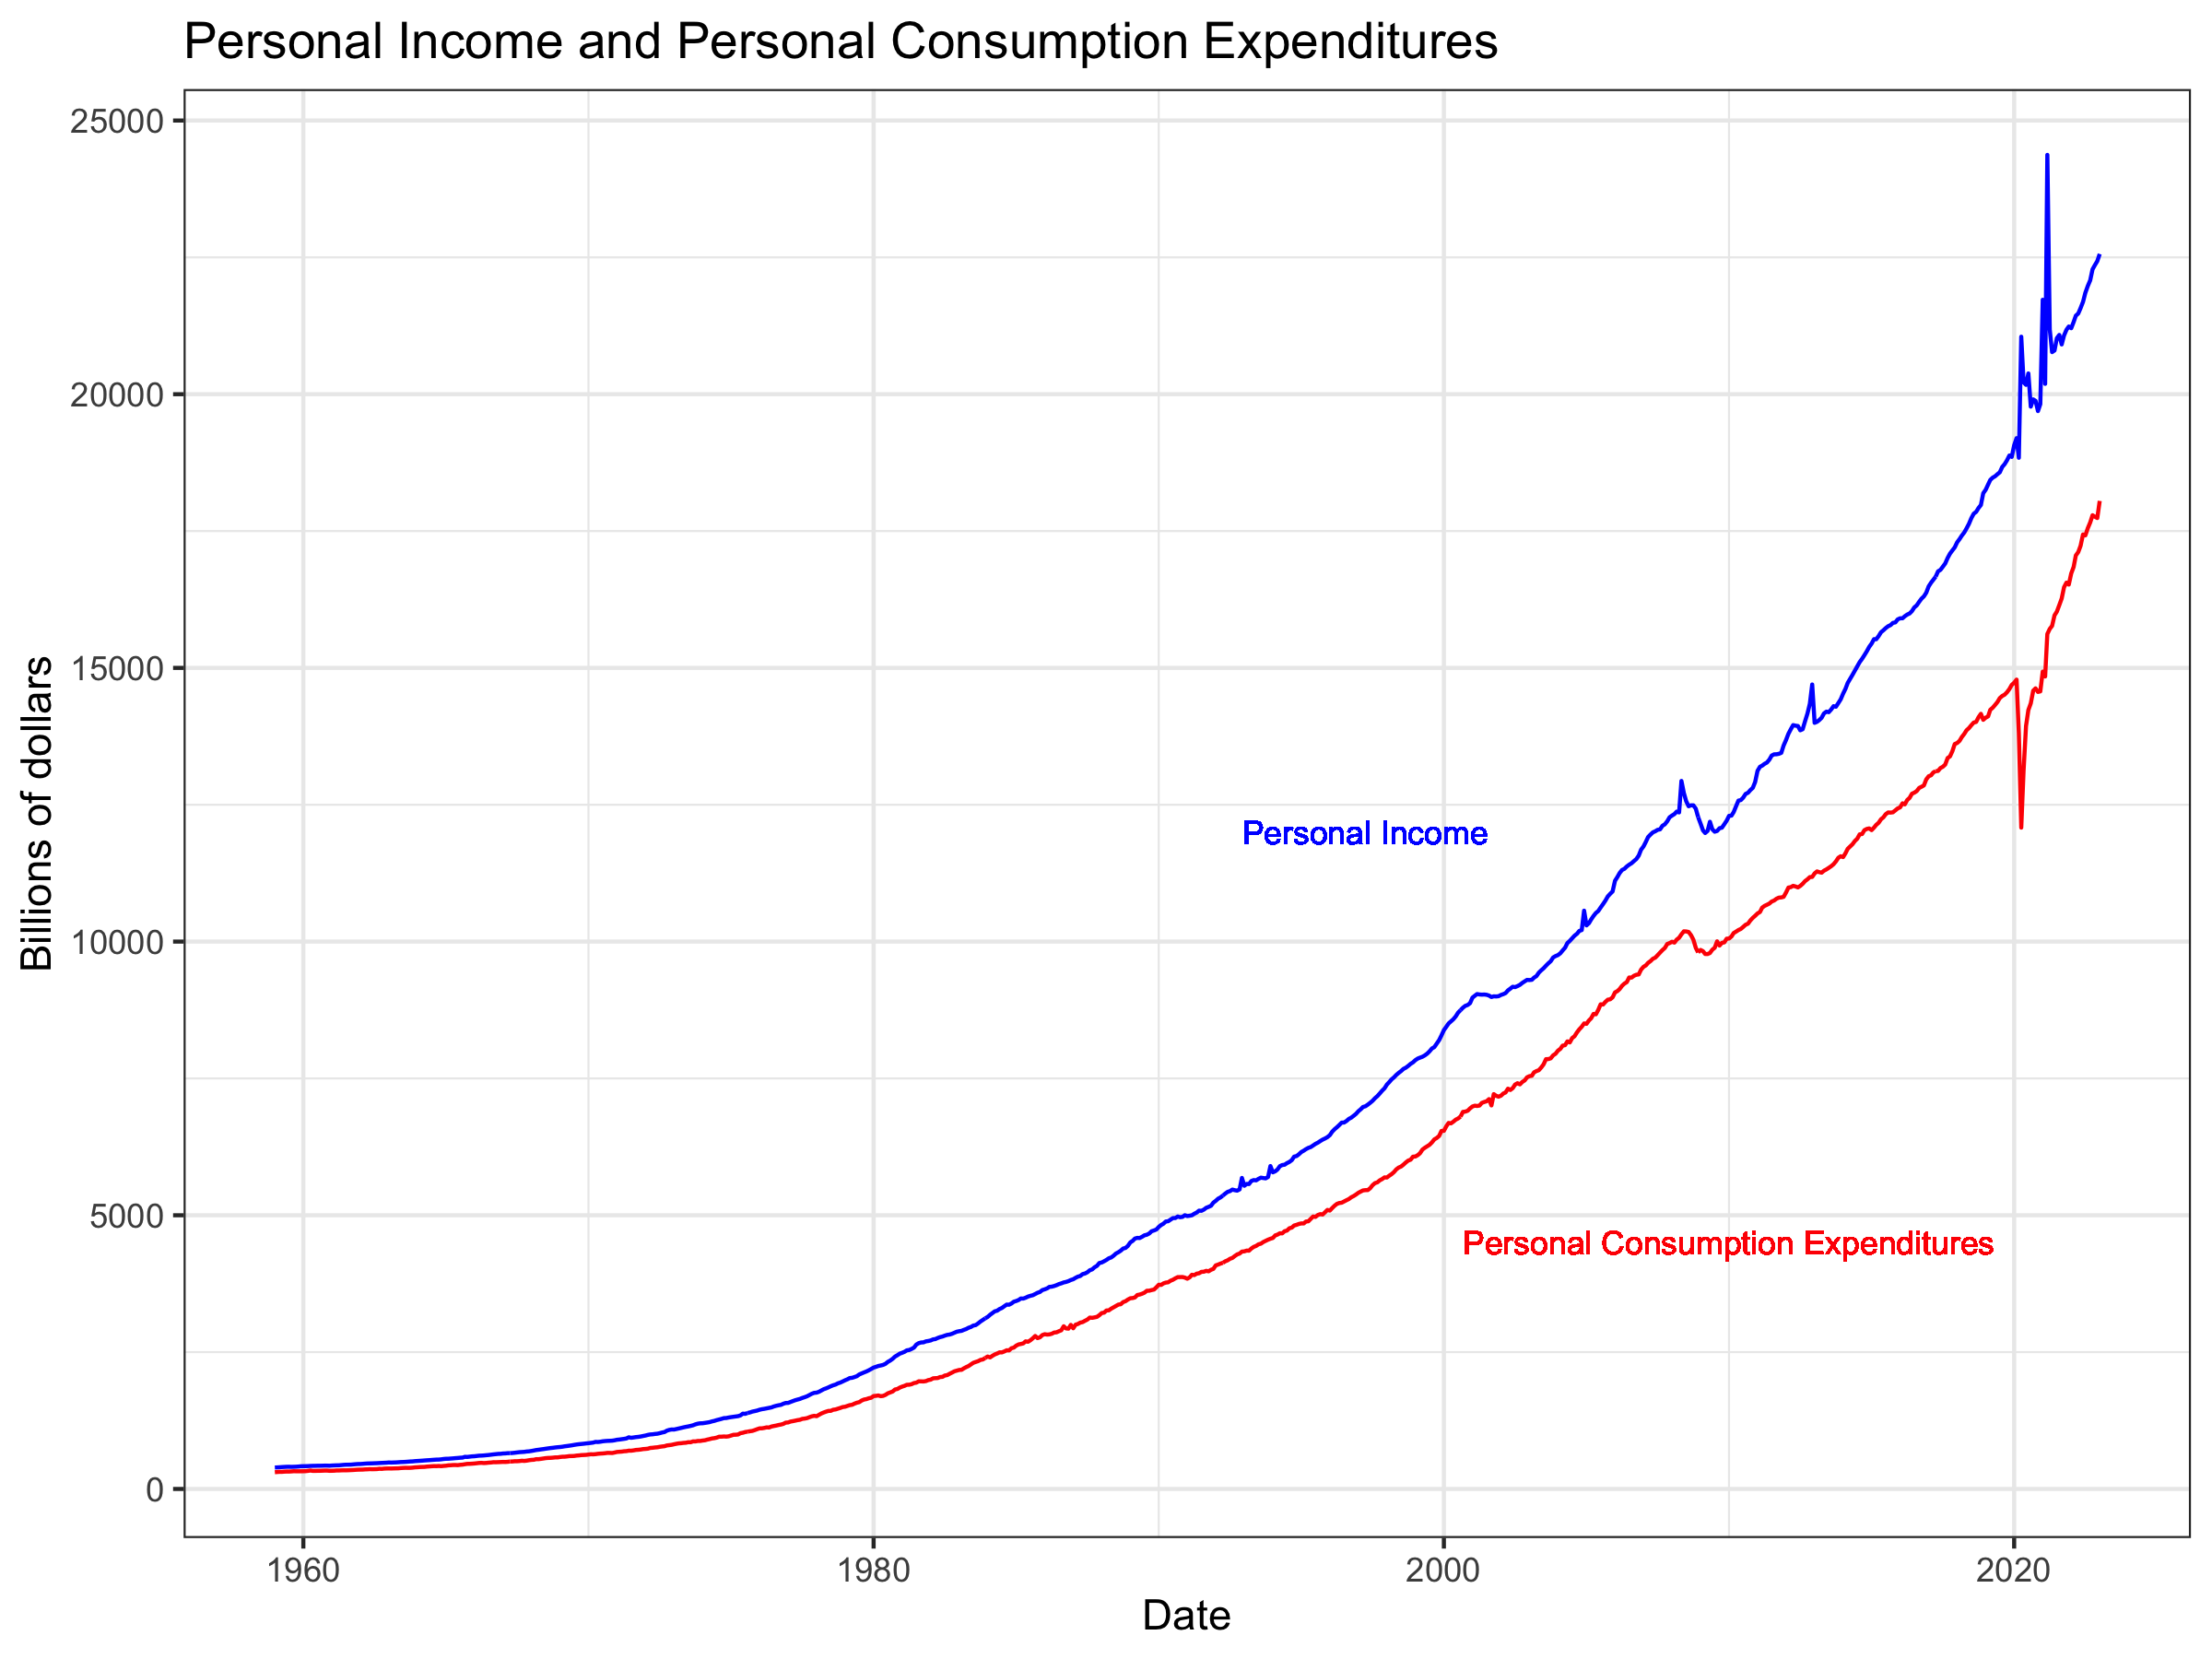
\includegraphics[width=0.8\textwidth]{PS6a_Gallart.png}
\end{figure}


\subsection{Pandemic Effects Subset}
This graph shows Personal Income and Personal Consumption Expenditure data from 2019 (pre-pandemic) to 2023. I wanted to make this a separate graph to be able to see the month to month changes more clearly. I did expect to see the biggest changes right at the beginning of the second quarter of 2020. I thought it was interesting that though income increased (likely because of stimulus checks to combat layoffs) consumption expenditure decreased. This was likely because of the transitional period to everything being online as well as in-person experiences, such as theaters and restaurants, were closed. It was interesting to see that CE stablized a quarter before income. This graph overall allows a closer look to the effects of the pandemic.

\begin{figure}[h]
\centering
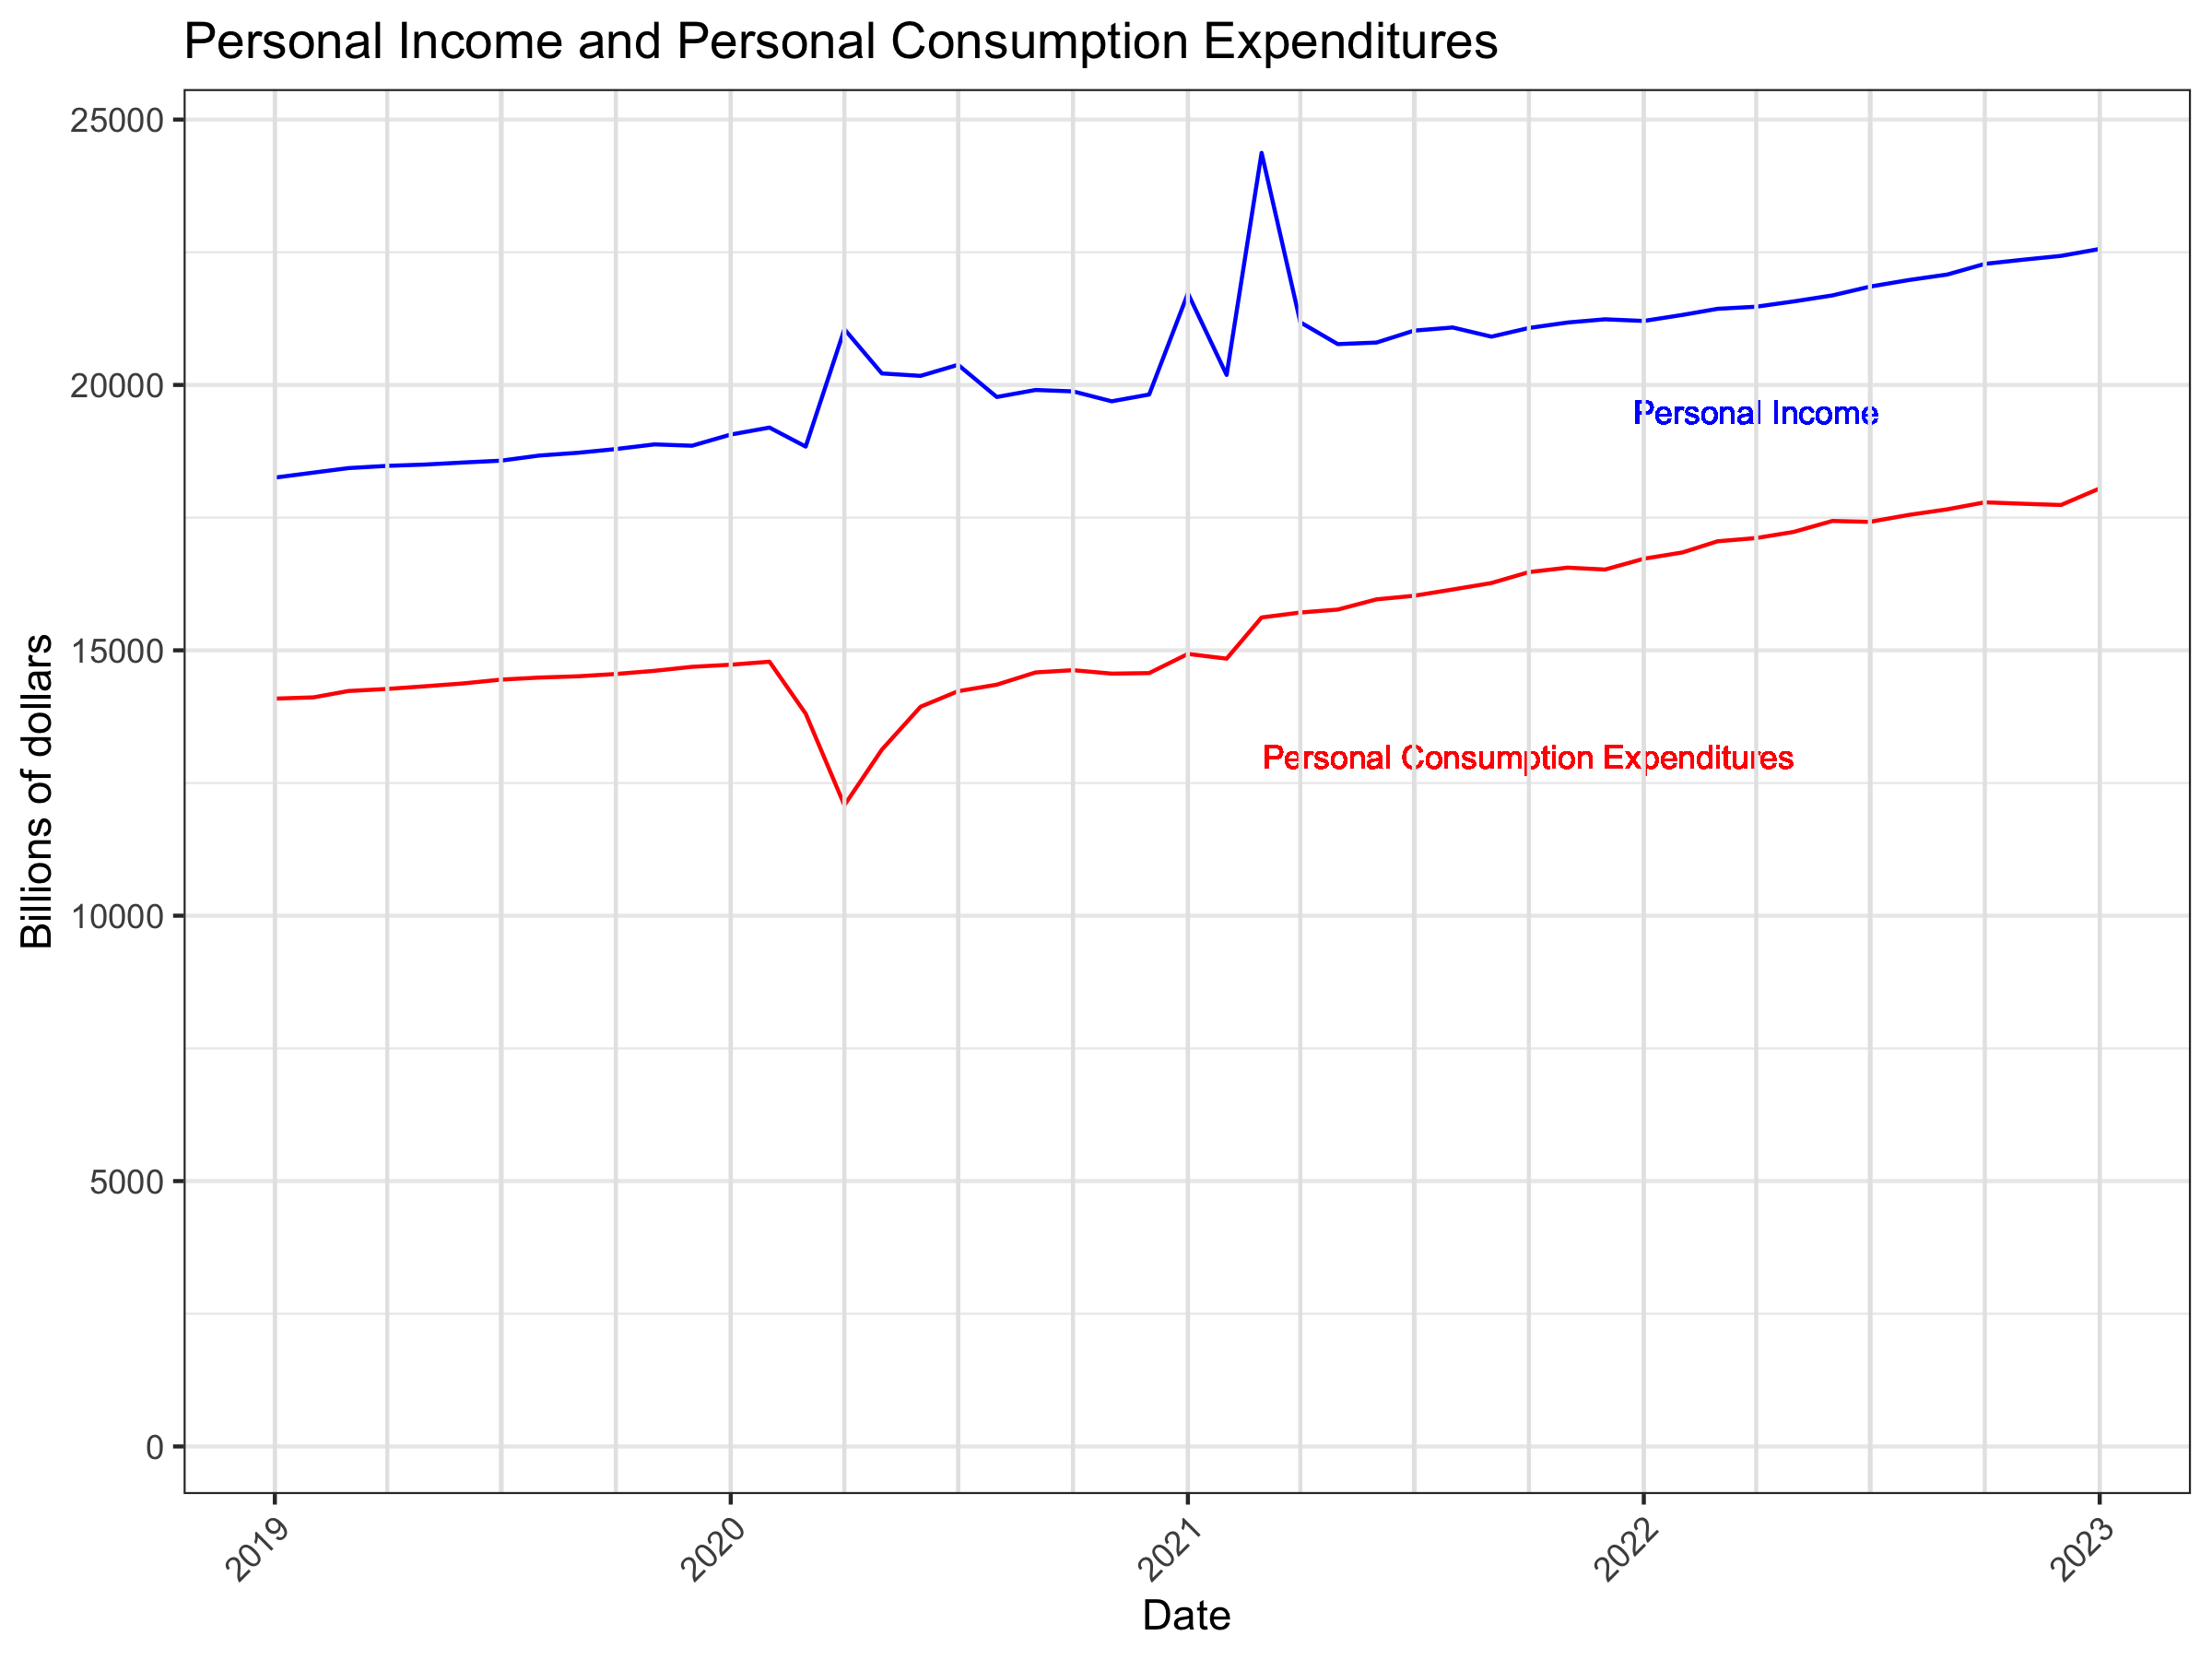
\includegraphics[width=0.8\textwidth]{PS6b_Gallart.png}
\end{figure}

\subsection{The Difference}
This graph shows the difference between Personal Income and Personal Consumption Expenditure data from FRED. I wanted to make this one after seeing the widening difference when looking at all the data. As you can see, the difference  increased pretty steadily until 2000. There were more fluctuations in the 2000s and 2010s, but it was still increasing overall. The pandemic drop was significant, as we saw broken down in the previous graph, but it recovered fairly quickly. The second drop surprised me, and the current difference was also not what I was expecting.

\begin{figure}[!t]
\centering
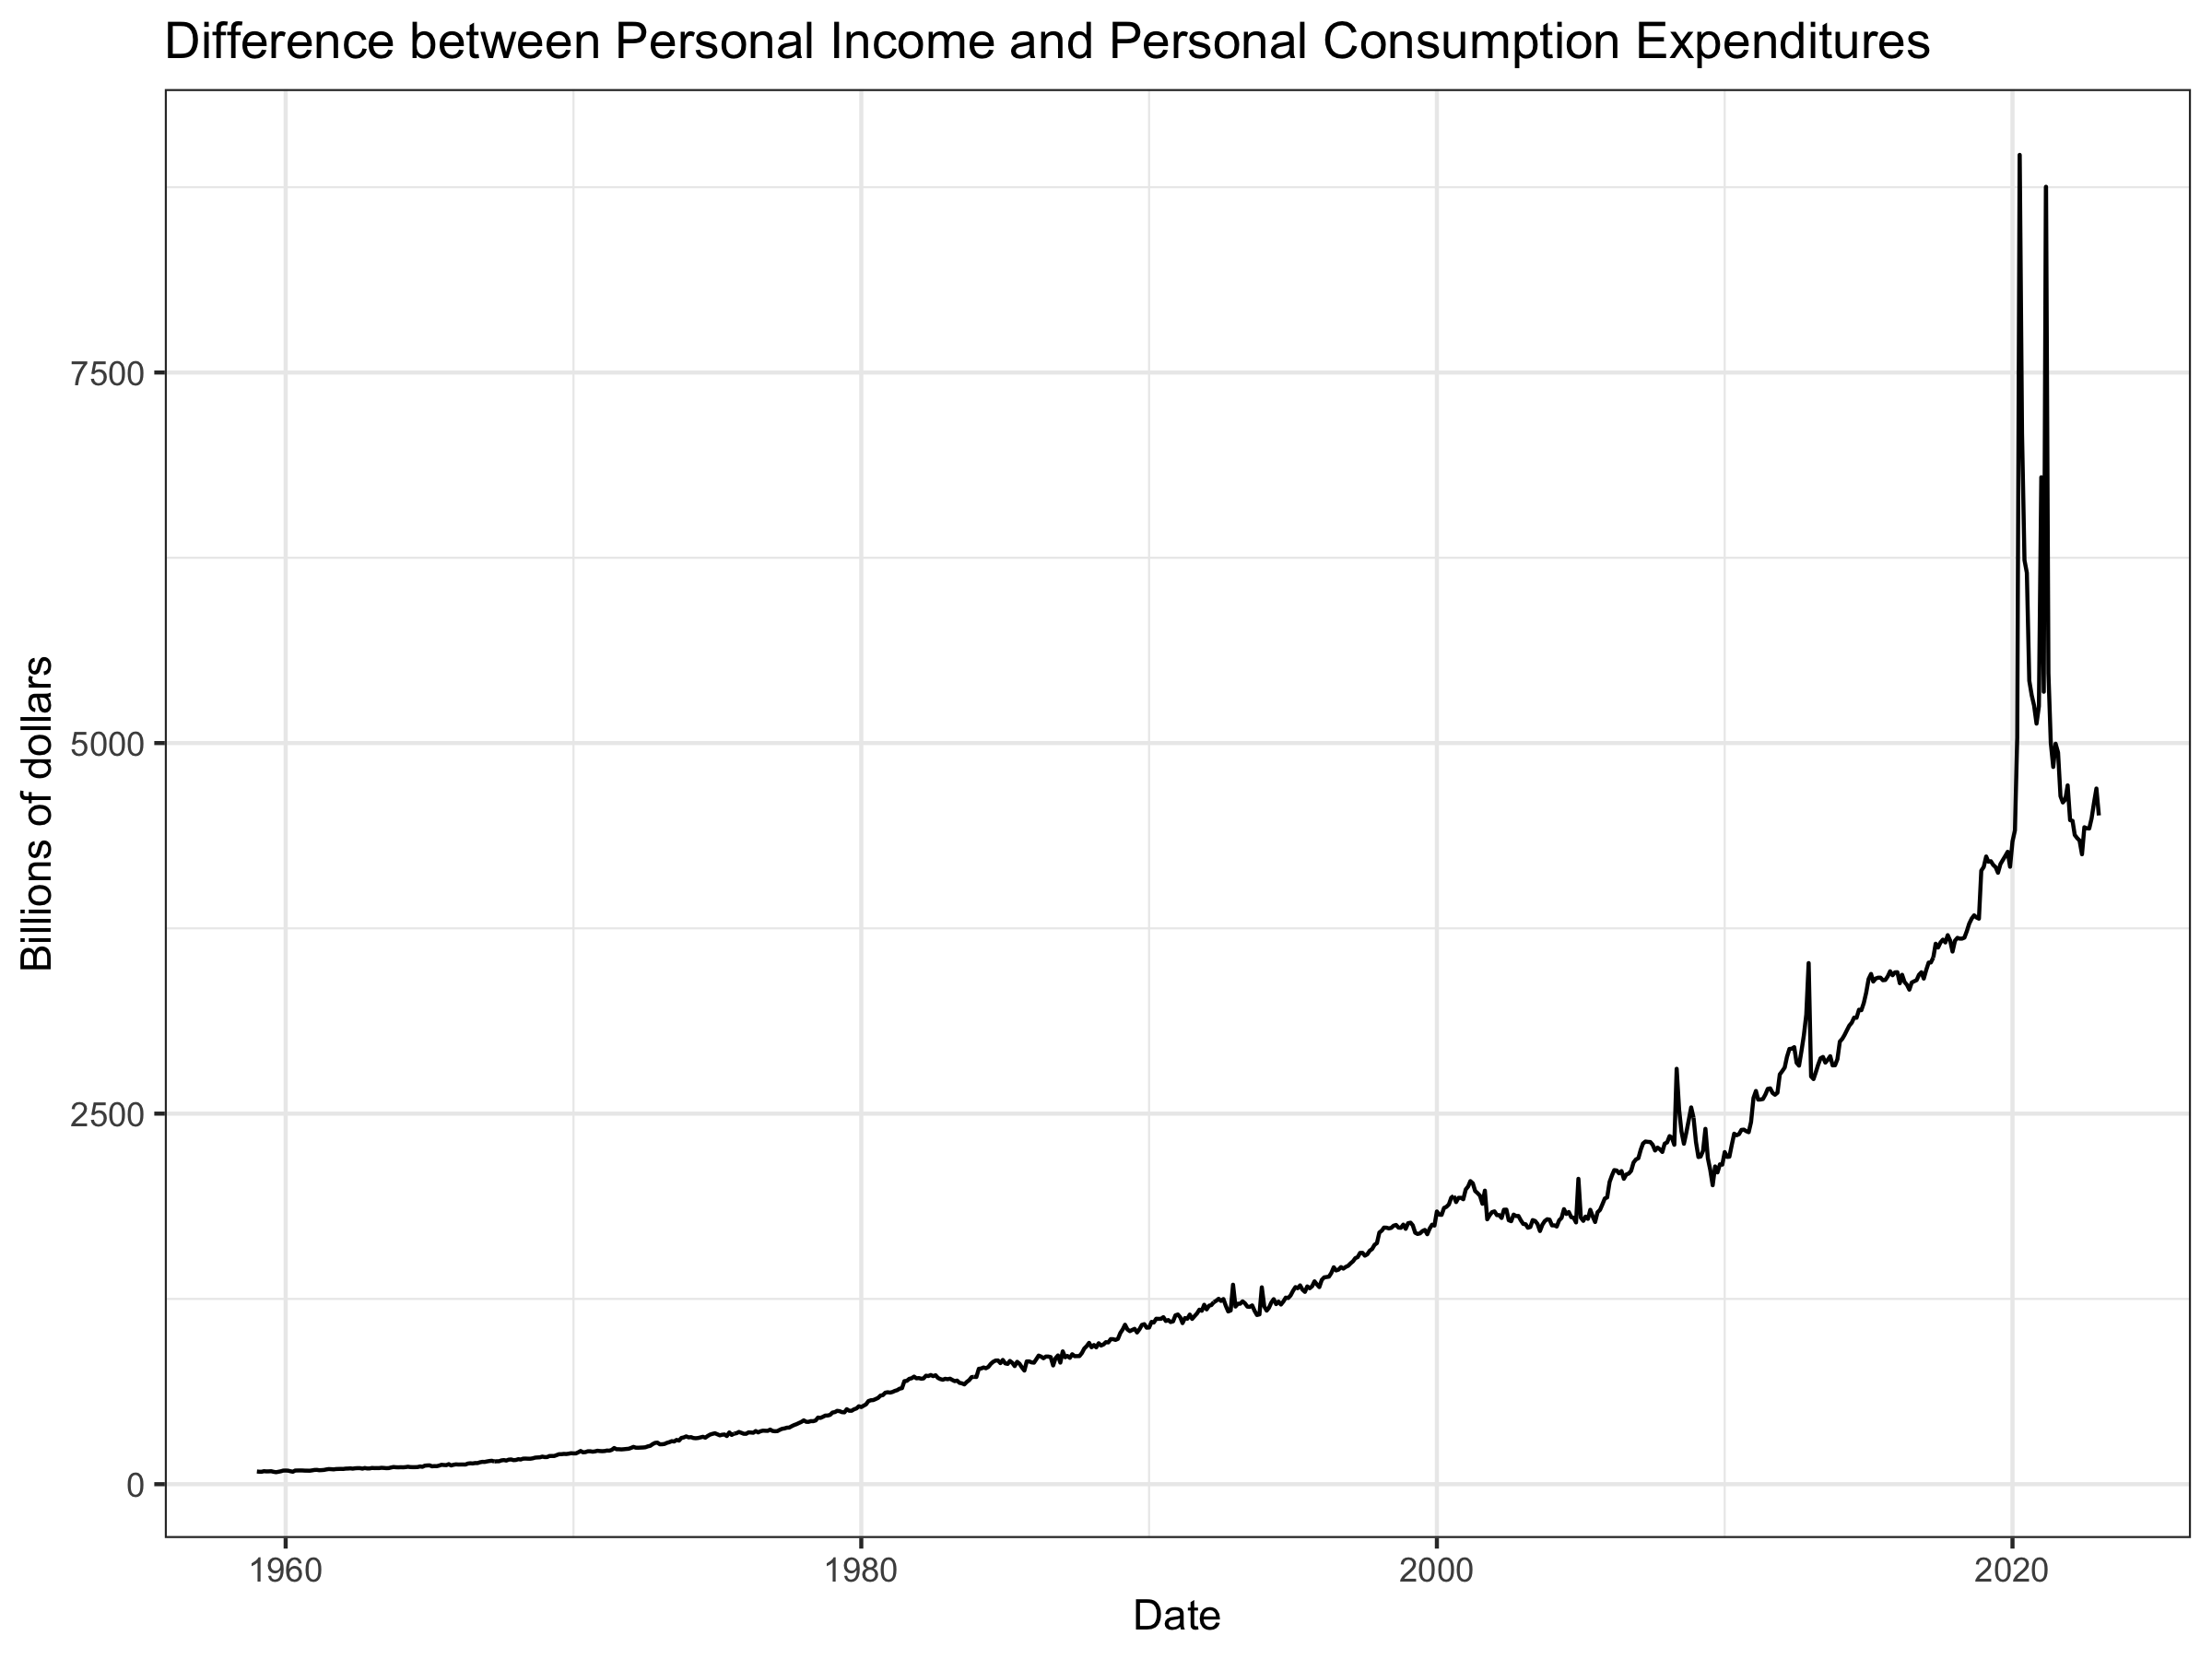
\includegraphics[width=0.8\textwidth]{PS6c_Gallart.png}

\end{figure}


\end{document}